\subsection{Разработка интерфейса взаимодействия}

Графический интерфейс пользователя, согласно выбору архитектуры клиент-сервер, основывается на технологии HTML + CSS + JavaScript с использованием Ajax запросов. 

\subsubsection{Разработка графа диалога}

Разработаем верхний уровень графа диалога с пользователем:
\begin{itemize}
\item \textbf{Главный экран} -- должен содержать элементы интерфейса для наиболее часто используемых функций АИС. Так как основной функцией АИС является поиск по новостным документам, то главный экран содержит рубрикатор, форму ввода поискового запроса и результат выполнения поискового запроса.
\item \textbf{Экран импорта} -- должен содержать элементы интерфейса для добавления документов в систему, а именно: форму ручного ввода, импорт архива документов и управление автоматизированным импортом документов из папки импорта.
\item \textbf{Экран экспорта} -- должен содержать элементы интерфейса для экспорта документов из системы.
\item \textbf{Экран управления} -- должен содержать элементы интерфейса для управления длительными операциями над индексом документов, над рубрикатором и другими действиями с предоставлением информации о прогрессе операции.
\item \textbf{Экран настроек} -- должен содержать элементы интерфейса для изменения и просмотра пользовательских настроек системы.
\item \textbf{Экран прогноза} -- должен содержать элементы интерфейса для отображения графиков активности новостных потоков, графики прогноза их активности, оценку качества прогноза и результирующую аналитическую функцию прогноза.
\end{itemize}

Обобщенный граф диалога представлен в графической части работы на листе <<Граф диалога с пользователем>>. %на рисунке~\ref{figure:dialog_generic}.

%\clearpage
%\begin{figure}[h!]
%\centering
%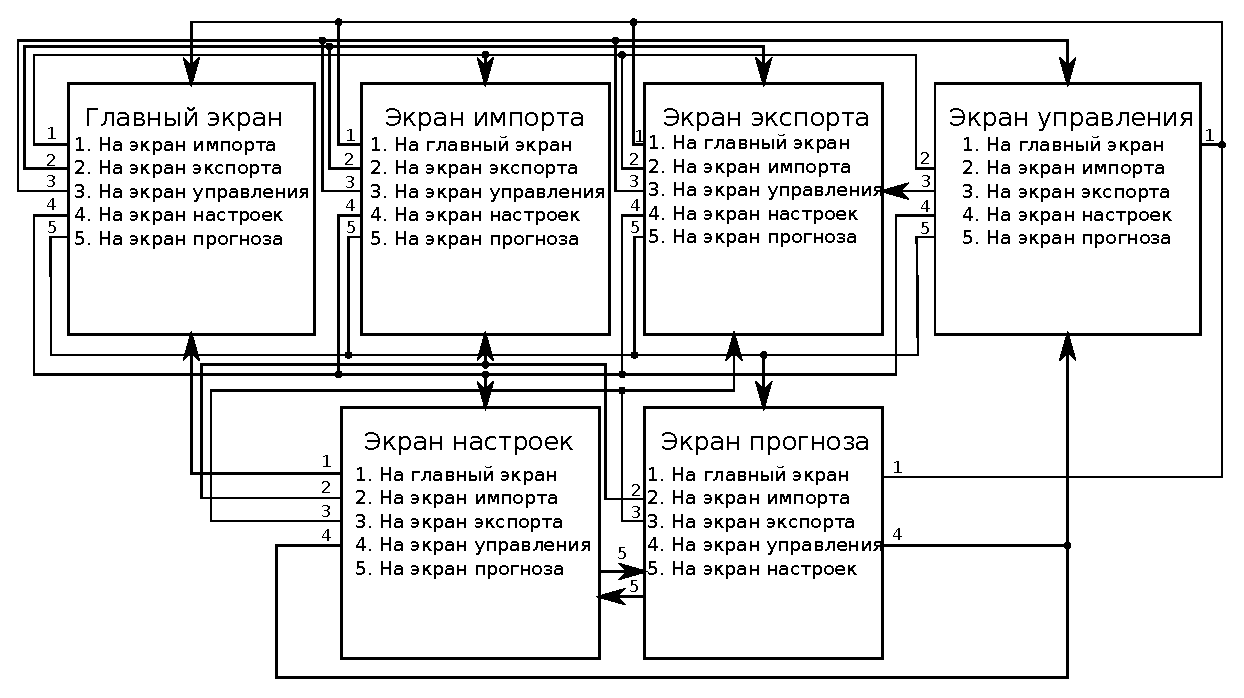
\includegraphics[angle=90,origin=c]{technology/dialog_generic}
%\caption{Обобщенный граф диалога взаимодействия с пользователем}
%\label{figure:dialog_generic}
%\end{figure}

\clearpage
\subsubsection{Разработка экранных форм}

При разработке экранных форму учитывались следующие требования к интерфейсу:
\begin{itemize}
\item Интерфейс должен быть удобен как для квалифицированного персонала, так и для новых пользователей АИС.
\item На каждом основном экране АИС должно присутствовать меню для перехода на другие экраны системы.
\item На каждом экране должны присутствовать только те элементы интерфейса, что необходимы для решения задачи, для которой экран предназначен.
\item Ввод данных должен быть интерактивным, то есть проводить проверку корректности вводимой информации и отображать причину ошибки в случае неправильно сформированных данных.
\end{itemize}

Основные экранные формы представлены в графической части проекта.

\clearpage
\subsection{Описание экранных форм}

\subsubsection{Главный экран}

  \begin{figure}[h!]
  \centering
  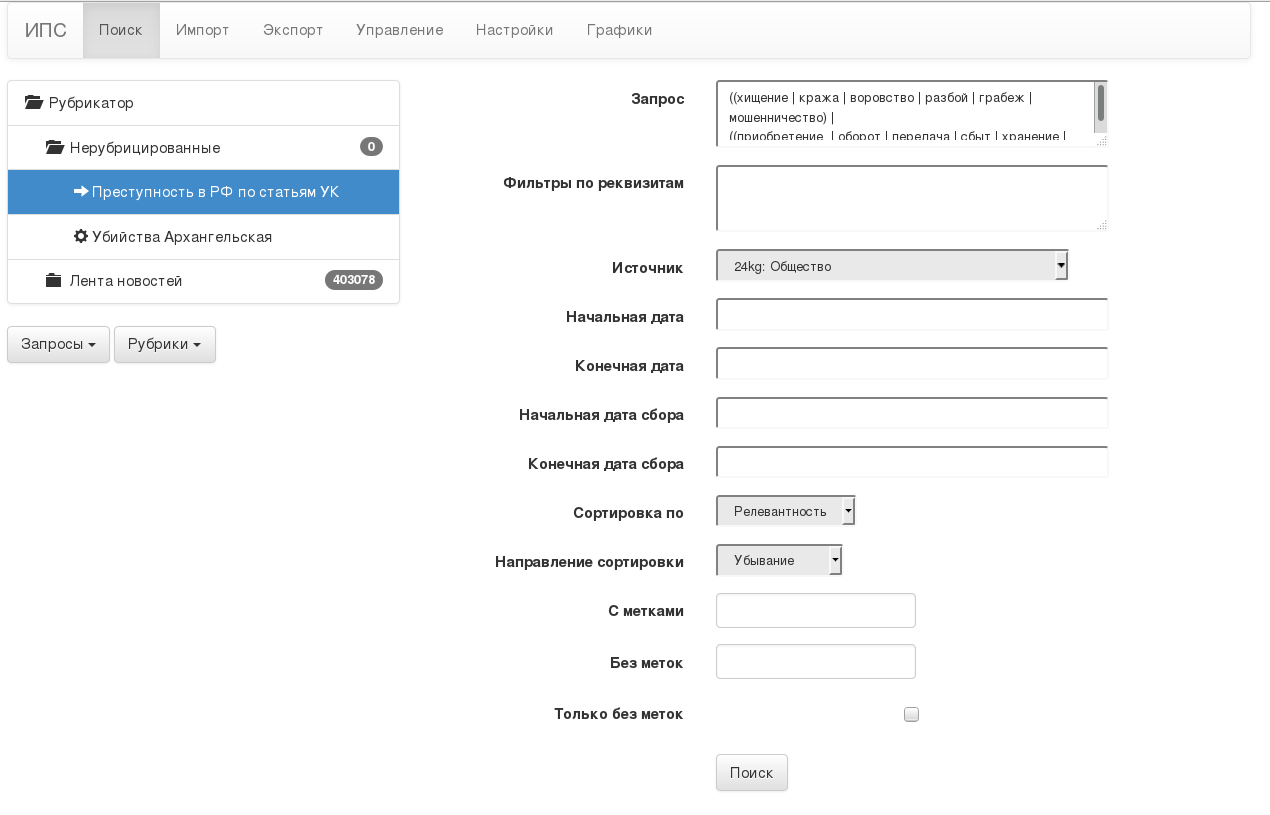
\includegraphics[width=0.9\linewidth]{technology/gui_main}
  \caption{Главный экран АИС}
  \label{figure:guiMain}
  \end{figure}

  На рис.~\ref{figure:guiMain} представлен вид главного экрана АИС. Экран содержит:
  \begin{itemize}
  \item Меню в верхней части экрана, через которое можно попасть на другие экраны системы.
  \item Рубрикатор в левой части экрана. Через рубрикатор пользователь может выбирать текущие категории документов, выбирать сохранённые запросы. Выпадающие панели под рубрикатором содержат действия над рубриками (создание, обновление, удаление, перемещение, экспорт из рубрики) и над сохранёнными запросами (создание, обновление, удаление). Рядом с названиями рубрик отображается количество документов в рубрике.
  \item Форма ввода запроса в правой части экрана. В форме присуствуют следующие поля:
  \begin{enumerate}
  \item Запрос -- тело формализованного запроса;
  \item Фильтры по реквизитам -- дополнительные ограничения на реквизиты документа;
  \item Источник -- выпадающий список из всех доступных источников документов;
  \item Начальная дата -- фильтрация по дате публикации документа. Задает начальное значение интервала;
  \item Конечная дата -- фильтрация по дате публикации документа. Задает конечное значение интервала;
  \item Начальная дата сбора -- фильтрация по дате сбора документа. Задает начальное значение интервала;
  \item Конечная дата сбора -- фильтрация по дате сбора документа. Задает конечное значение интервала;
  \item Сортировка по -- указание реквизита документа, по которому будет проводиться сортировка;
  \item Направление сортировки -- указание направления сортировки, по убыванию или по возрастанию;
  \item С метками -- перечисление меток документа, которые должны у него присутствовать;
  \item Без меток -- перечисление меток документа, которые должны у него отсутствовать;
  \item Только без меток -- специальный признак, при активации которого поиск будет проводиться только по документам, у которых нет никаких меток;
  \end{enumerate}

  \end{itemize}

  \begin{figure}[h!]
  \centering
  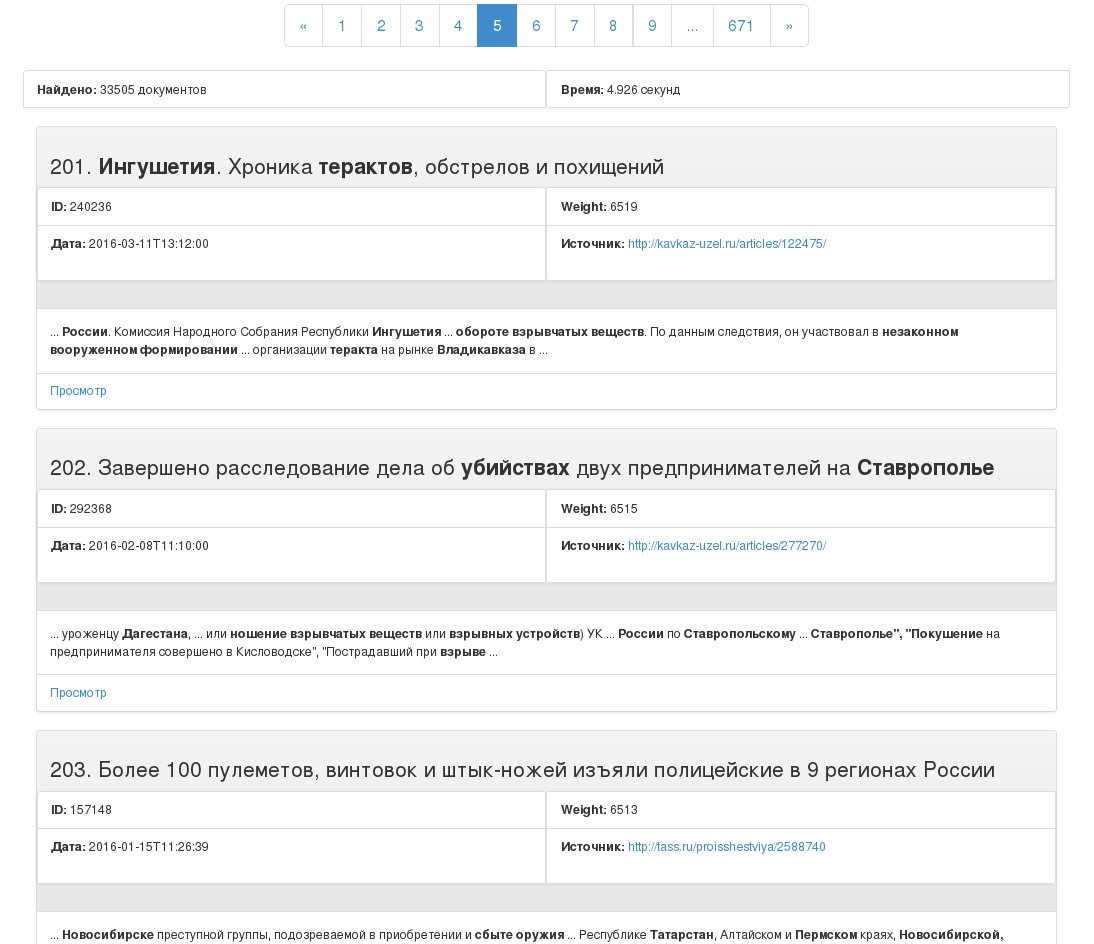
\includegraphics[width=0.9\linewidth]{technology/gui_main_results}
  \caption{Главный экран АИС, поисковая выдача}
  \label{figure:guiMainResults}
  \end{figure}

  После нажатия на кнопку <<Поиск>> в нижней части экрана пользователю отображается вторая часть данного экрана с поисковой выдачей (рис.~\ref{figure:guiMainResults}). Поисковая выдача может содержать множество документов, поэтому экран содержит кнопки перехода по страницам. Каждый элемент выдачи содержит название документа, его основные реквизиты и кусок текста, который подходит под заданный формализованный запрос. 

  \begin{figure}[h!]
  \centering
  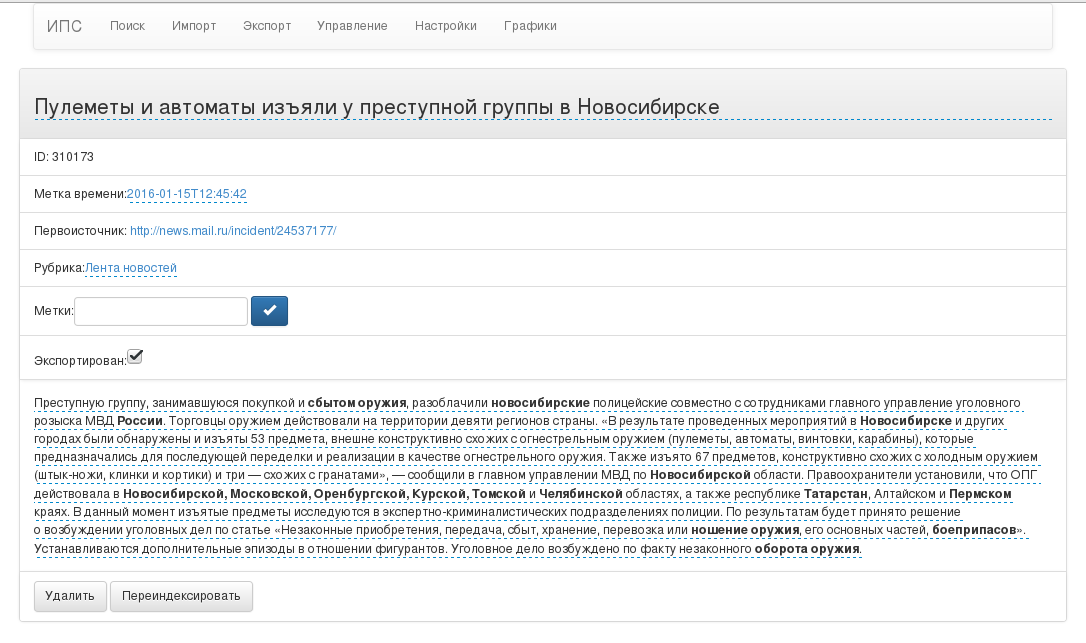
\includegraphics[width=0.9\linewidth]{technology/gui_main_document}
  \caption{Просмотр полного документа}
  \label{figure:guiMainDocument}
  \end{figure}

  Документ в элементе поисковой выдачи можно просмотреть отдельно с помощью ссылки <<Просмотр>> в нижней части элемента выдачи. Вид страницы документа представлен на рис.~\ref{figure:guiMainDocument}. Подробный вид документа содержит значения всех реквизитов, а также предоставляет возможность удаления или переиндексирования документа. Каждый реквизит, кроме идентификатора и источника, можно отредактировать путем щелчка мышкой на данных реквизита и ввода новых во всплывающем элементе ввода. Текст документа подсвечен согласно последнему выполненному запросу.

\clearpage
\subsubsection{Экран импорта}

  \begin{figure}[h!]
  \centering
  
\includegraphics[width=0.9\linewidth]{technology/gui_import}
  \caption{Экран импорта документов}
  \label{figure:guiImport}
  \end{figure}

  На рис.~\ref{figure:guiImport} представлен вид экрана импорта документов. Экран содержит:
  \begin{itemize}
  \item Меню в верхней части экрана, через которое можно попасть на другие экраны системы.
  \item Кнопку перехода в ручной режим -- ввод документов через форму ввода поштучно, представлено на рис.~\ref{figure:guiImportSingle}.
  \item Кнопку перехода в режим архива -- отправка архива с несколькими документами. Интерфейс этого режима предназначен для загрузки очень объемных архивов с отображением процесса загрузки. Режим представлен на рис.~\ref{figure:guiImportArchive}.
  \item Кнопку запуска импорта из папки импорта -- при нажатии на эту кнопку происходит ручное инициирование сканирования папки импорта на новые документы.
  \end{itemize}

  \begin{figure}[h!]
  \centering
  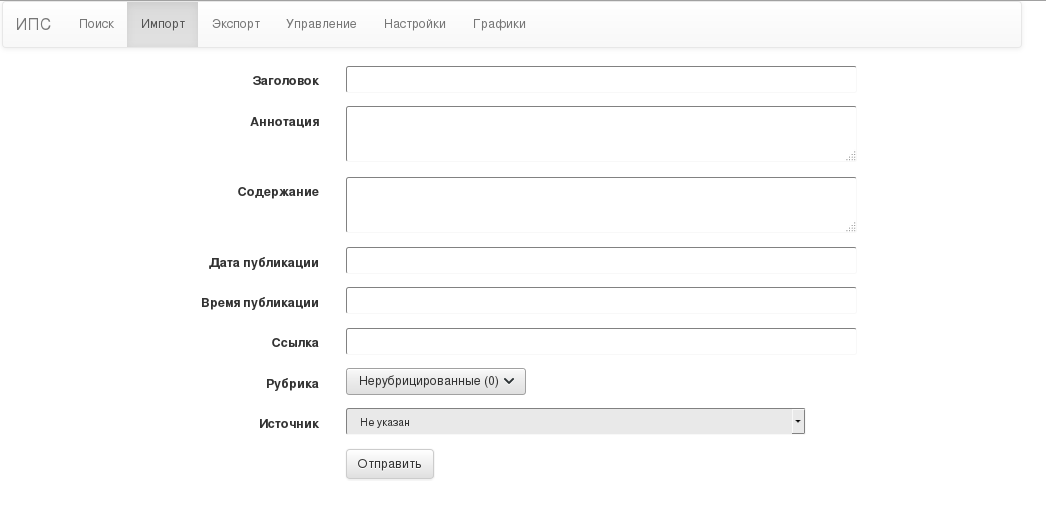
\includegraphics[width=0.9\linewidth]{technology/gui_import_single}
  \caption{Экран импорта документов, ручной режим}
  \label{figure:guiImportSingle}
  \end{figure}

  \begin{figure}[h!]
  \centering
  
\includegraphics[width=0.9\linewidth]{technology/gui_import_archive}
  \caption{Экран импорта документов, режим архива}
  \label{figure:guiImportArchive}
  \end{figure}

\clearpage
\subsubsection{Экран экспорта}

  \begin{figure}[h!]
  \centering
  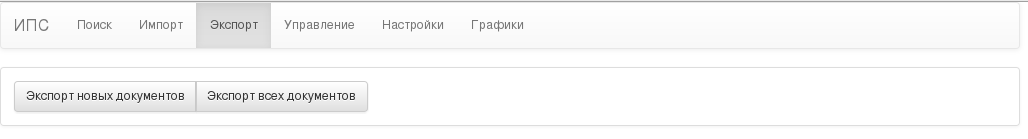
\includegraphics[width=0.9\linewidth]{technology/gui_export}
  \caption{Экран экспорта документов}
  \label{figure:guiExport}
  \end{figure}

  На рис.~\ref{figure:guiExport} представлен вид экрана экспорта документов. Экран содержит:
  \begin{itemize}
  \item Меню в верхней части экрана, через которое можно попасть на другие экраны системы.
  \item Кнопка запуска полного экспорта, при нажатии на которую начинается полный экспорт документов.
  \item Кнопка запуска инкрементального экспорта, при нажатии на которую начнется экспорт только еще не экспортированных документов.
  \end{itemize}

  При нажатии на любую из кнопок стартует операция система, список которых можно посмотреть на экране управления. Также во время экспорта на всех экранах системы отображается информационный элемент (рис.~\ref{figure:guiExportInfo}), а после завершения экспорта на экране экспорта отображается список готовых архивов, которые пользователь может скачать и перенести на другую развернутую АИС <<Волхв>>.

  \begin{figure}[h!]
  \centering
  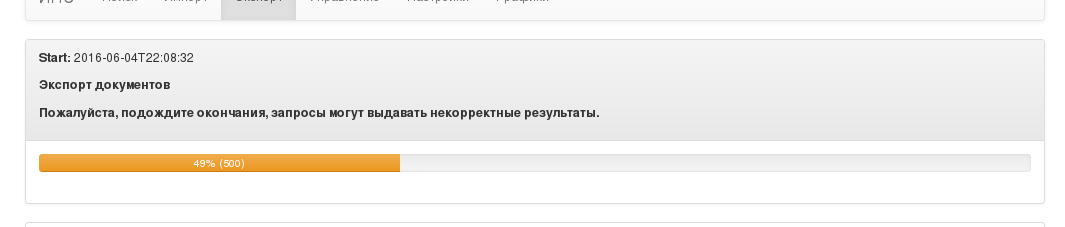
\includegraphics[width=0.9\linewidth]{technology/gui_export_info}
  \caption{Информационный элемент, который показывается на всех экранах АИС во время операции экспорта.}
  \label{figure:guiExportInfo}
  \end{figure}

\clearpage
\subsubsection{Экран управления}

  \begin{figure}[h!]
  \centering
  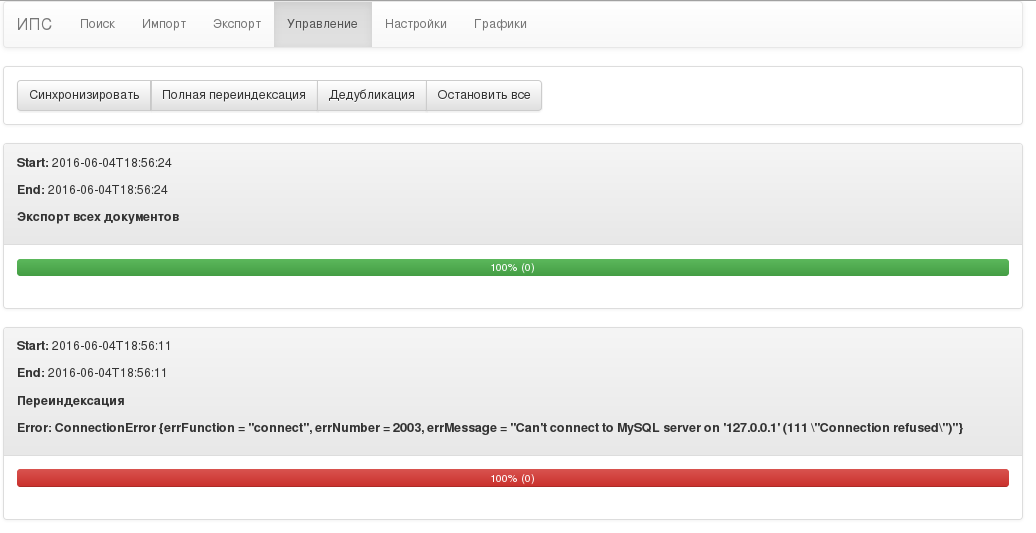
\includegraphics[width=0.9\linewidth]{technology/gui_resync}
  \caption{Экран управления операциями АИС}
  \label{figure:guiResync}
  \end{figure}

  На рис.~\ref{figure:guiResync} представлен вид экрана управления операциями АИС. Экран содержит:
  \begin{itemize}
  \item Меню в верхней части экрана, через которое можно попасть на другие экраны системы.
  \item Панель управления с кнопками запуска операций над базой документов: 
    \begin{enumerate}
      \item Синхронизировать -- запуск операции синхронизации индекса с базой документов, данная операция необходима при неполадках в системе для восстановления целостности индекса.
      \item Полная переиндексация -- запуск операции переиндексации базы документов, в отличии от синхронизации переиндексация удаляет весь индекс и перестраивает его с нуля. Данная операция нужна, когда меняются настройки индекса и для корректной его работы необходимо провести перестройку индекса.
      \item Дедубликация -- запуск операции удаления дублей из базы данных документов. При неаккуратном обращении с системой возможна ситуация, когда в базу были загружены дубли документов, данная операция находит и удаляет такие дубли.
      \item Остановить все -- прекращает выполнение всех операций, запущенных в данный момент.
    \end{enumerate}
  \item Список операций, запущенных или уже завершившихся. Для каждой операции отображается дата начала и конца работы. При аварийном завершении отображается текст ошибки и панель прогресса подсвечивается красным. При успешном завершении панель прогресса отображается зеленым цветом, а операции в процессе выполнения обозначаются желтым цветом.
  \end{itemize}

\clearpage
\subsubsection{Экран настроек}

\begin{figure}[h!]
\centering
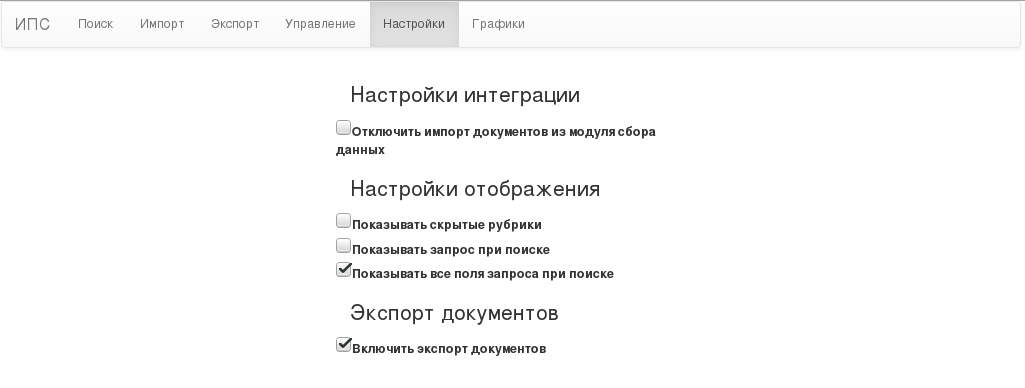
\includegraphics[width=0.9\linewidth]{technology/gui_options}
\caption{Экран настроек АИС}
\label{figure:guiOptions}
\end{figure}

На рис.~\ref{figure:guiOptions} представлен вид экрана настроек АИС. Экран содержит:
\begin{itemize}
\item Меню в верхней части экрана, через которое можно попасть на другие экраны системы.
\item Список настроек системы, каждая из которых представлена элементом <<checkbox>>:
\begin{enumerate}
  \item Отключение автоматического импорта документов из папки импорта. Необходимо при проведении технических работ над индексом, при которых нежелательно поступление новых документов в базу данных.
  \item Показ скрытых рубрик. Каждая рубрика может иметь признак скрытости и не отображаться пользователю через web-интерфейс. Такие рубрики используются для интеграции с другими системами и позволяют делать сохраненные формализованные запросы  и рубрики для использования другими сервисами.
  \item Показ запроса при поиске. При включенном признаке система будет показывать полученный поисковый запрос перед выборкой документов, пример такого запроса представлен на рис.~\ref{figure:guiOptionsQuery}.
  \item Показ всех полей при поиске. При отключенном признаке система не будет показывать редко используемые поля в форме ввода поискового запроса.
  \item Включить экспорт документов. При отключенном признаке система скроет все элементы, относящиеся к функциональности экспорта документов. Данная опция полезна для реплик АИС, для которых экспорт документов не используется, а только мешает пользователям.
\end{enumerate}
\end{itemize}

\begin{figure}[h!]
\centering
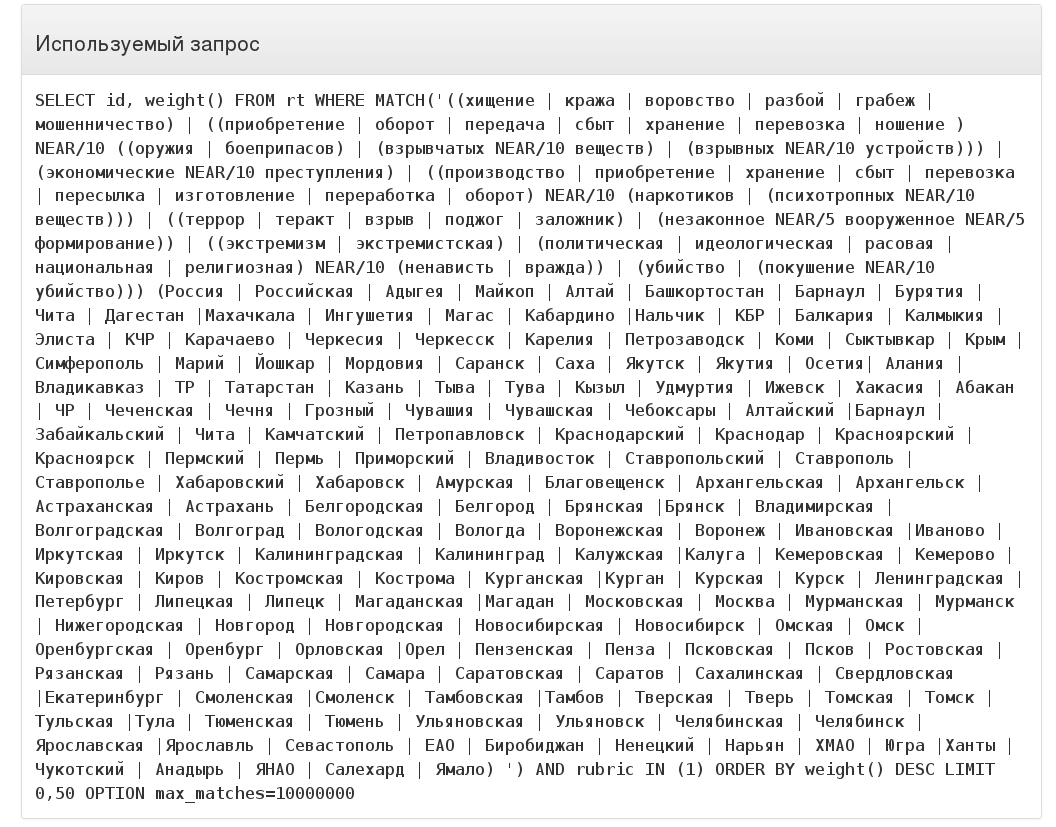
\includegraphics[width=0.9\linewidth]{technology/gui_options_query}
\caption{Элемент вывода запроса при поиске}
\label{figure:guiOptionsQuery}
\end{figure}


\clearpage
\subsubsection{Экран прогнозирования} 

\begin{figure}[h!]
\centering
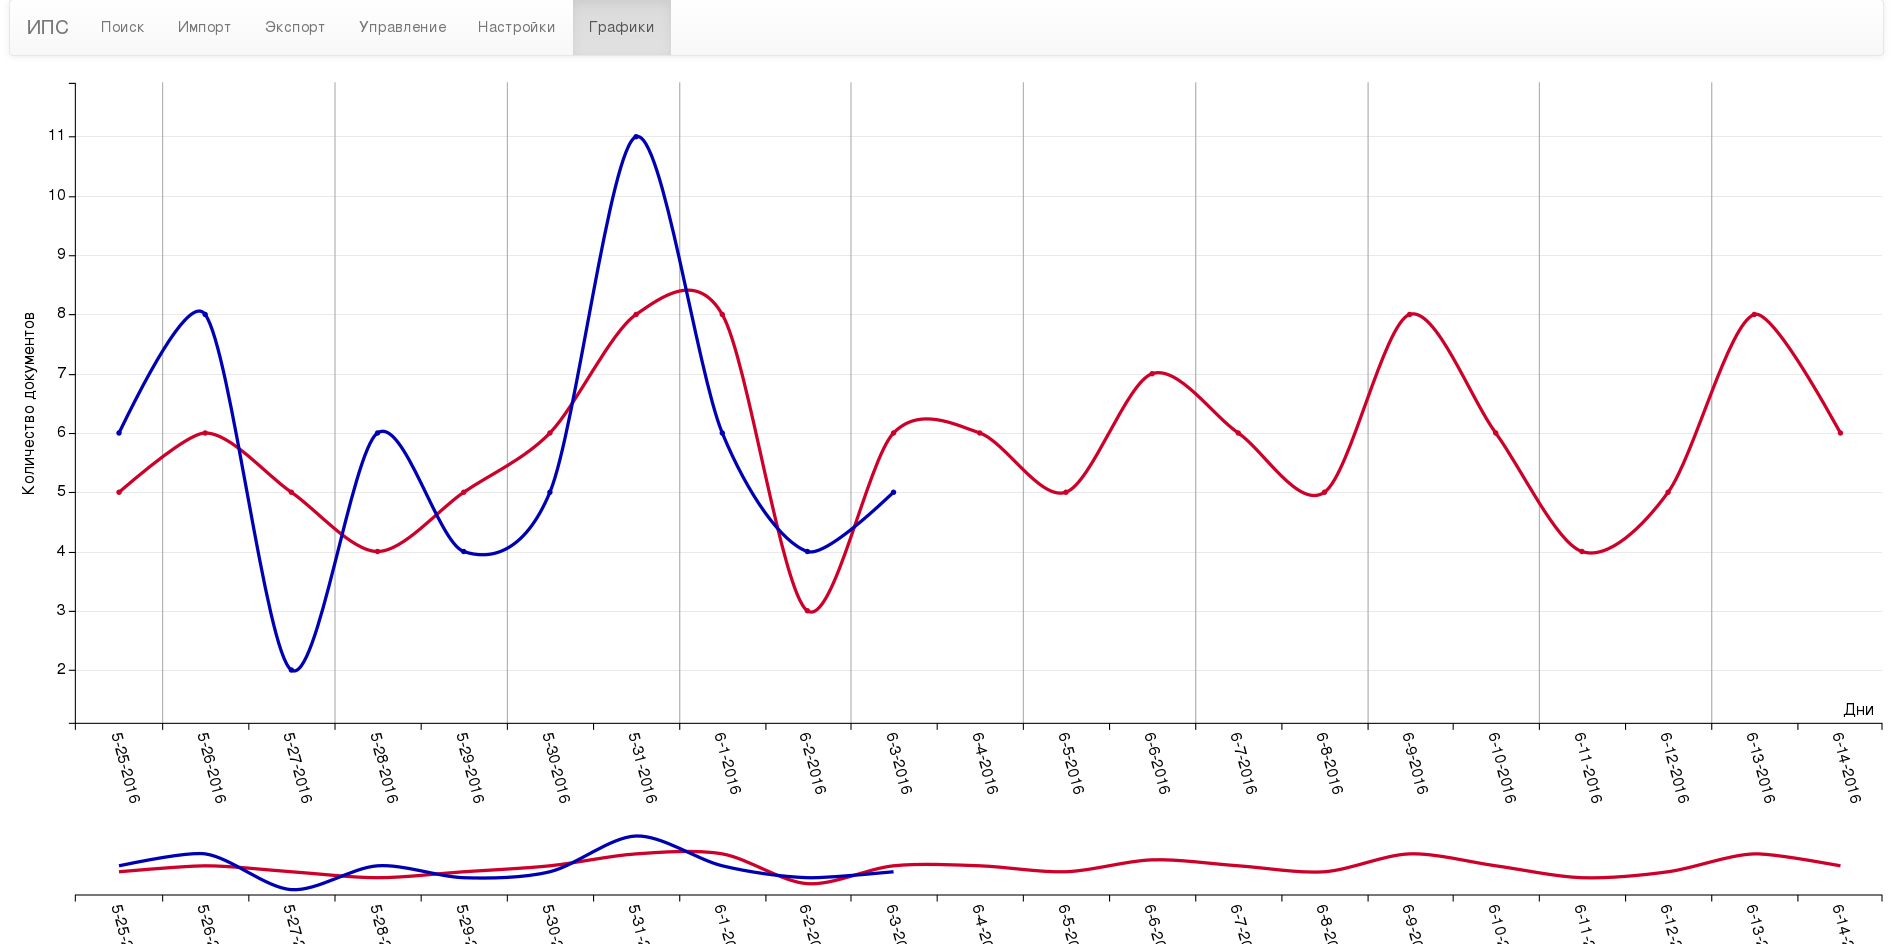
\includegraphics[width=0.9\linewidth]{technology/gui_predict1}
\caption{Экран прогнозирования АИС, часть 1}
\label{figure:guiPredict2}
\end{figure}

\begin{figure}[h!]
\centering
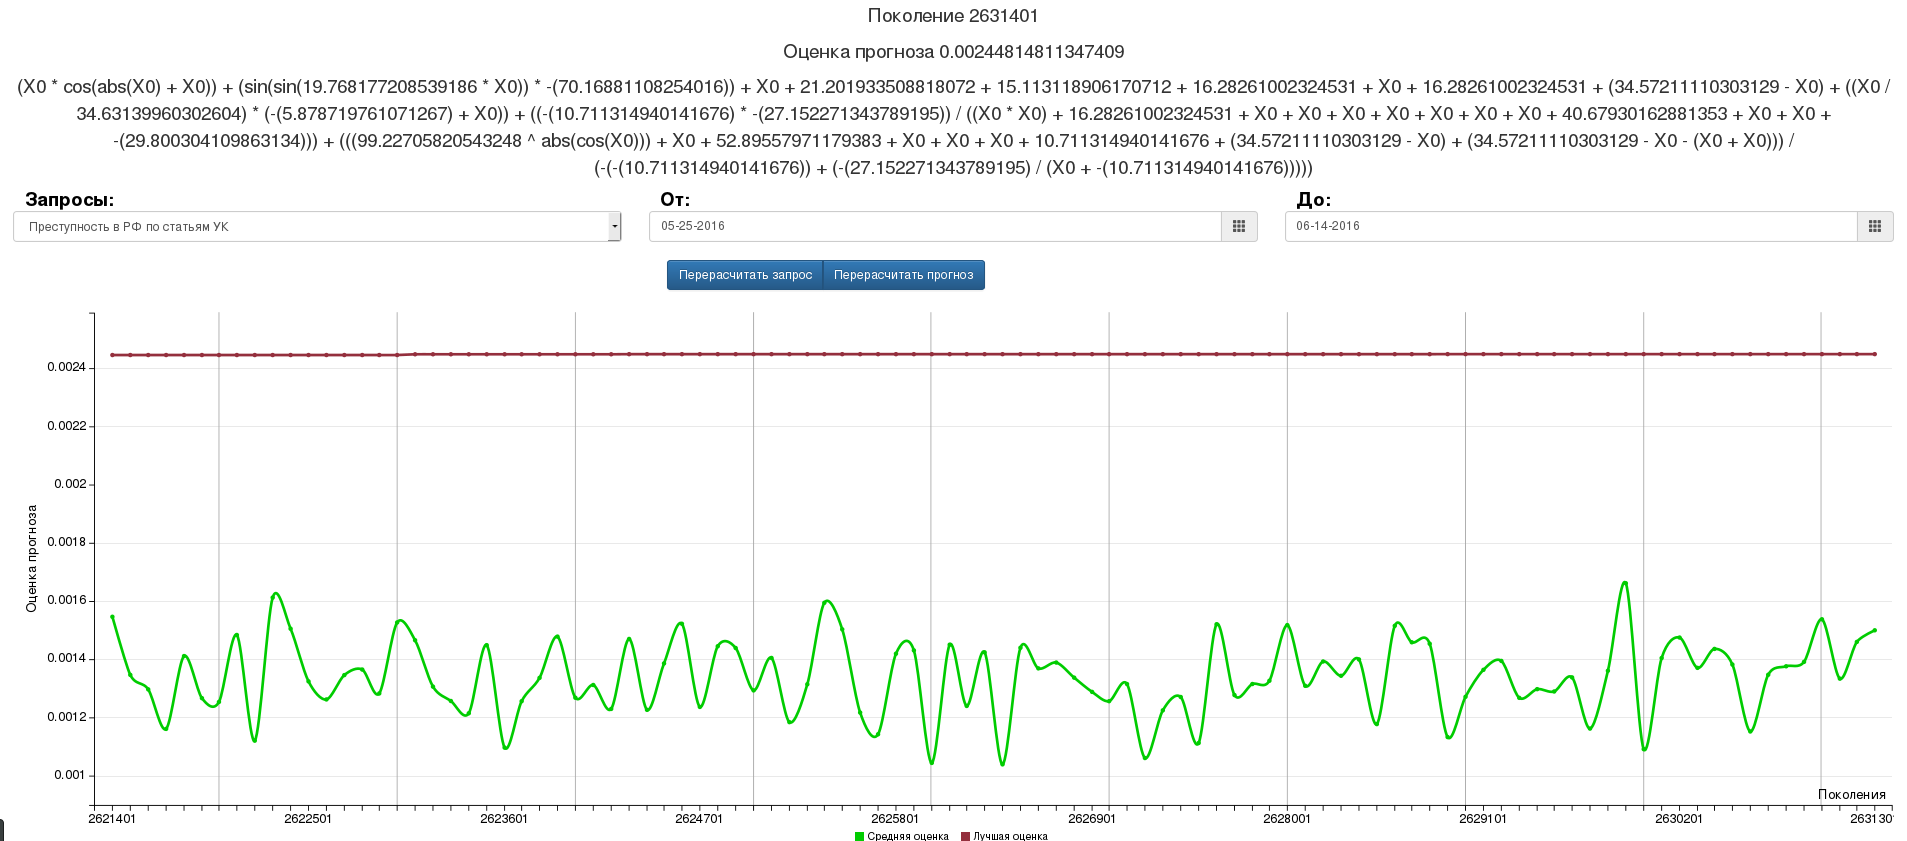
\includegraphics[width=0.9\linewidth]{technology/gui_predict2}
\caption{Экран прогнозирования АИС, часть 2}
\label{figure:guiPredict1}
\end{figure}

На рис.~\ref{figure:guiPredict1} и рис.~\ref{figure:guiPredict2} представлен вид экрана прогнозирования АИС. Экран содержит:
\begin{itemize}
\item Меню в верхней части экрана, через которое можно попасть на другие экраны системы.
\item Элемент графиков, который содержит два подграфика:
\begin{enumerate}
  \item Синий график -- значения количества документов, удовлетворяющих сохраненному запросу по дням. 
  \item Красный график -- график прогноза количества документов по дням, в том числе и ретроспективный прогноз для оценки качества прогнозирования.
\end{enumerate}
\item Миниатюра графиков -- отображение всего рассматриваемого периода времени. Пользователь может выбрать интервал внутри миниатюры, и верхний график подстроится для отображения под заданный интервал времени.
\item Число поколений прогноза -- отображает количество поколений, прошедших в эволюционном алгоритме, с начала прогнозирования.
\item Количественная оценка качества прогнозирования -- среднеквадратичное отклонение прогноза от реальных данных.
\item Аналитическая формула прогноза -- аналитическая функция, полученная в результате символьной регрессии на основе эволюционных алгоритмов.
\item Вспомогательный график для оценки качества прогноза:
\begin{enumerate}
\item Коричневая линия отображает лучшие значение функции приспособленности от поколения популяций. Данная функция должна монотонно не убывать при низменности реальных данных.
\item Зеленая линия отображает среднее значение функции приспособленности от поколения популяций. Данная функция должна быть ниже коричневой, что свидетельствует от генетическом разнообразии популяций.
\end{enumerate}
\end{itemize}
